%%%%%%%%%%%%%%%%%%%%%%%%%%%%%%%%%%%%%%%%%%%%%%%%%%%%%%%%%%%%%%%%%%%%%%%%%%%%%%%%
% Author: Daniela Pointinger <dpointinger.itsb-m2013@fh-salzburg.ac.at>
%
% Fachhochschule Salzburg, Campus Urstein
% Studiengang: ITS Master, berufsbegleitend (itsb-m2013)
%%%%%%%%%%%%%%%%%%%%%%%%%%%%%%%%%%%%%%%%%%%%%%%%%%%%%%%%%%%%%%%%%%%%%%%%%%%%%%%%

\documentclass{beamer}
\usepackage[ngerman]{babel}	% Jep, wir machen es in deutsch
\usepackage[utf8]{inputenc}	% Und ja, UTF8 ist cool
\usepackage{graphicx}		% Wir brauchen auch Grafiken!
\usepackage{hyperref}

\usecolortheme{beetle}
\usetheme{Szeged}	% Übers Theme lässt sich noch streiten

% Präsentationstitel (das in [] steht in der Fußzeile)
\title[]{Software-Engineering\\Bahn Zahlsystem}

% Restliche Metadata
\author{Daniela Pointinger \& Michael Haslauer \\\& Stefan Winkler \& Johannes Briewasser}
\institute{FH-Salzburg, Studiengang ITSB-M}
\date{\today}

\begin{document}

% Titelseite
\begin{frame}
	\titlepage
\end{frame}

% Inhaltsverzeichnis
\begin{frame}{Übersicht}
	\tableofcontents
\end{frame}

\section{Intro}
\begin{frame}{Bahn Zahlsystem}
	\begin{itemize}
		\item Entwicklung eines Zahlsystems für Bahnkunden
		\item Online-Shop für Speisewagen
		\item einfache Bedienung (z.B. per App)
		\item mehrere Zahlungsmöglichkeiten
	\end{itemize}
\end{frame}

\section{Requirements-Engineering}
\begin{frame}{Requirements-Engineering}
	\begin{block}{Metamodell}
		Entwicklung einer eigenen DSL für die Erstellung von Requirements und Use Cases
	\end{block}
	
	\begin{block}{Gründe für ein Metamodell}
	\begin{itemize}
		\item Standardisierte Form für einen Use Case
		\item Definition von Modalverben
	\end{itemize}
	\end{block}
\end{frame}

\begin{frame}{Metamodell}
	\begin{center}
		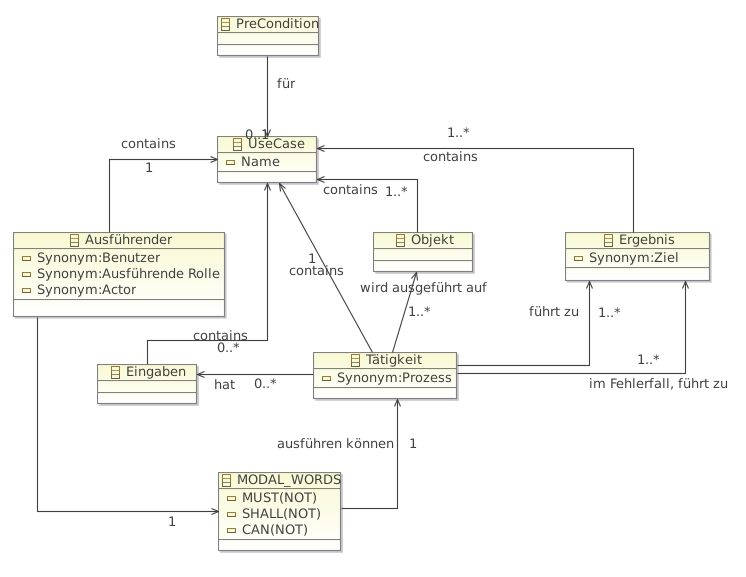
\includegraphics[width=0.85\textwidth]{img/metamodell.png}
	\end{center}
\end{frame}

\begin{frame}{Use Case Vorlage}
	\begin{center}
		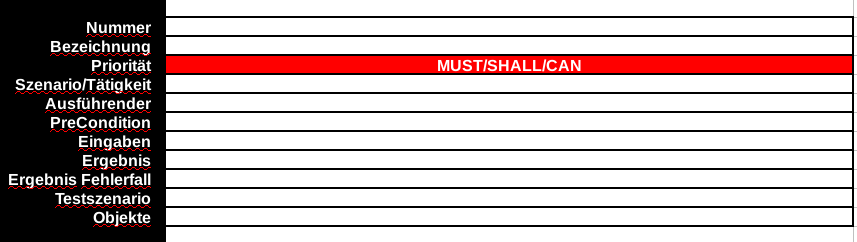
\includegraphics[width=\textwidth]{img/use-case-vorlage.png}
	\end{center}
\end{frame}

\begin{frame}{Use Case Beispiel 1}
	\begin{center}
		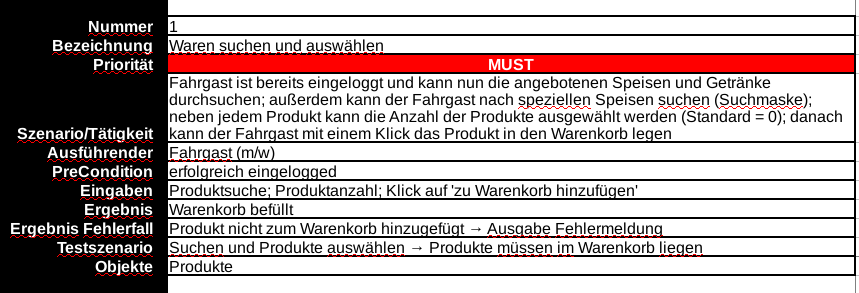
\includegraphics[width=\textwidth]{img/use-case-bsp-1.png}
	\end{center}
\end{frame}

\begin{frame}{Use Case Beispiel 2}
	\begin{center}
		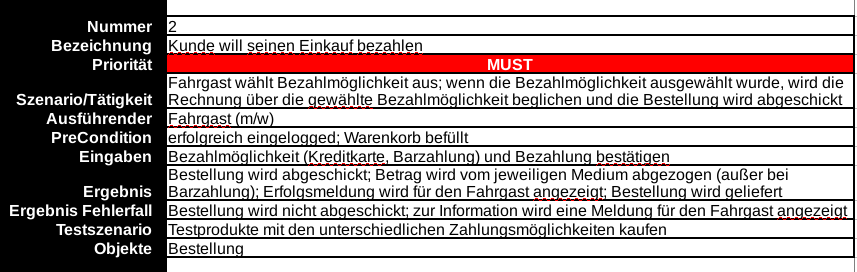
\includegraphics[width=\textwidth]{img/use-case-bsp-2.png}
	\end{center}
\end{frame}

\section{Architektur}
\begin{frame}{Softwarearchitektur}
	\begin{itemize}
		\item Auswahl des Architekturmodells -$>$ Schichtenmodell
	\end{itemize}
	\begin{block}{Gründe für das Schichtenmodell}
		\begin{itemize}
			\item Trennung von Aufgabenbereichen
			\item separate Entwicklung jeder Schicht
			\item dadurch sind unterschiedliche Entwicklungsteams möglich
		\end{itemize}
	\end{block}
\end{frame}

\begin{frame}{Schichtenmodell}
	\begin{itemize}
		\item Domänenobjekte und Peristenz
		\item Business-Logik
		\item Benutzeroberfläche
		\item Anbindung von Drittsystemen
	\end{itemize}
\end{frame}

\begin{frame}
	\begin{figure}[H]
		\centering	
		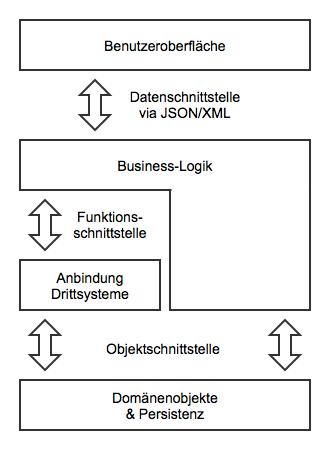
\includegraphics[width=0.5\textwidth]{img/architektur.png}
	\end{figure}
\end{frame}

\end{document}
